%Chapter 2 - Literature Review

\chapter{Literature Review} % Main chapter title
\label{Chapter2} % For referencing the chapter elsewhere, use \ref{Chapter1} 

%----------------------------------------------------------------------------------------
%----------------------------------------------------------------------------------------
\section{Early home computer era} \label{sec: Early home computer era}
 
Mid-1970s to late-1980s was an interesting period in the history of computers. It marked the first time computers were designed and marketed for personal use in the home; the early home computer era. The term \textit{home computer} is ambiguous, and not defined by any Standard. In this thesis it is taken to be synonymous with a microcomputer or a personal computer (PC) from the era. A PC is classified in the \textit{Proceedings of the IEEE} from 1984 by Gupta, A. and Toong, H. as a computer that fulfils all of the following characteristics 
\cite{RN24}: 

\begin{enumerate}
\item The computer cost less than US\$5000 at the time of sale.\\
\item The computing power is provided by a microprocessor from the era. \\
\item The computer is sold through mass-marketing channels. \\
\item The computer can run a wide range of programs for varied fields such as industry, business, education and at home; it is not designed for a single purpose or a single type of user.
\item The computer can handle at least one high-level language , such as BASIC, Fortran, or COBOL.
\end{enumerate}

Since the discovery of semiconductors in the 1940s, there have been continuous efforts and advances in making electronic devices smaller, more powerful and cheaper. 1958 saw the first working Integrated Circuit (IC, also called a microchip or chip), continuing this trend 
\cite{RN36}. By 1965, Moore was talking about the observation mentioned above, which came to be popularly known as "Moore's Law" 
\cite{RN33}. In 1971, Intel developed the first microprocessor; the 4-bit 4004 on a single IC 
\cite{RN37}, shown in figure \ref{Intel4004}. A microprocessor is an entire CPU within an IC or a few ICs. The following year Intel released the more powerful 8-bit 8008 microprocessor. Then in 1974 the 8080 was released 
\cite{RN38}. 

\begin{figure} \begin{center}
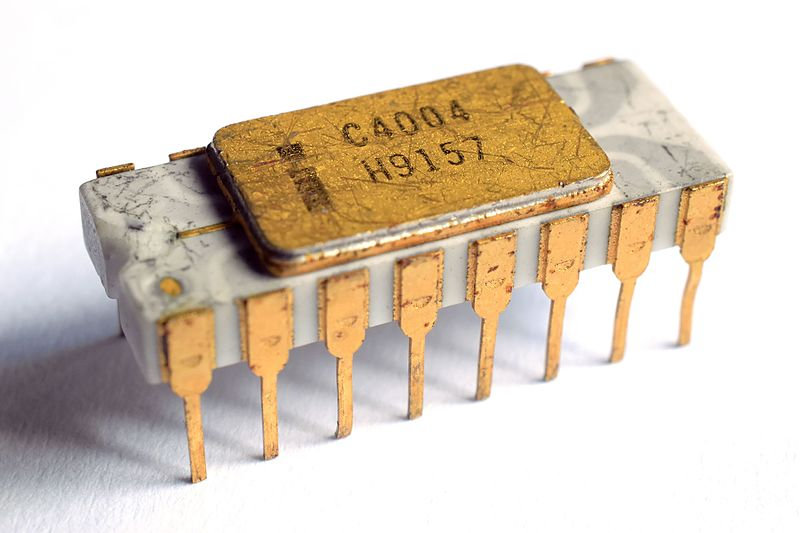
\includegraphics[width=.3\linewidth]{pics/intel_4004} 
\end{center} 
\caption{Intel 4004 microprocessor, an entire CPU on a single chip; the first microprocessor. Released in 1971.\\ \textit{\small{Picture courtesy of Thomas Nguyen}}}
\label{Intel4004}
\end{figure} 

It seems a tipping point had now been reached, the manufacturing cost of computers was low enough, their size was small enough and their performance was high enough that some manufacturers decided to start designing and marketing them to personal users. In 1974, MITS released what can be considered the first market-successful home computer 
\cite{RN41}, the Altair 8800 which used an 8080 microprocessor shown in figure \ref{Altair8800}.

\begin{figure} \begin{center}
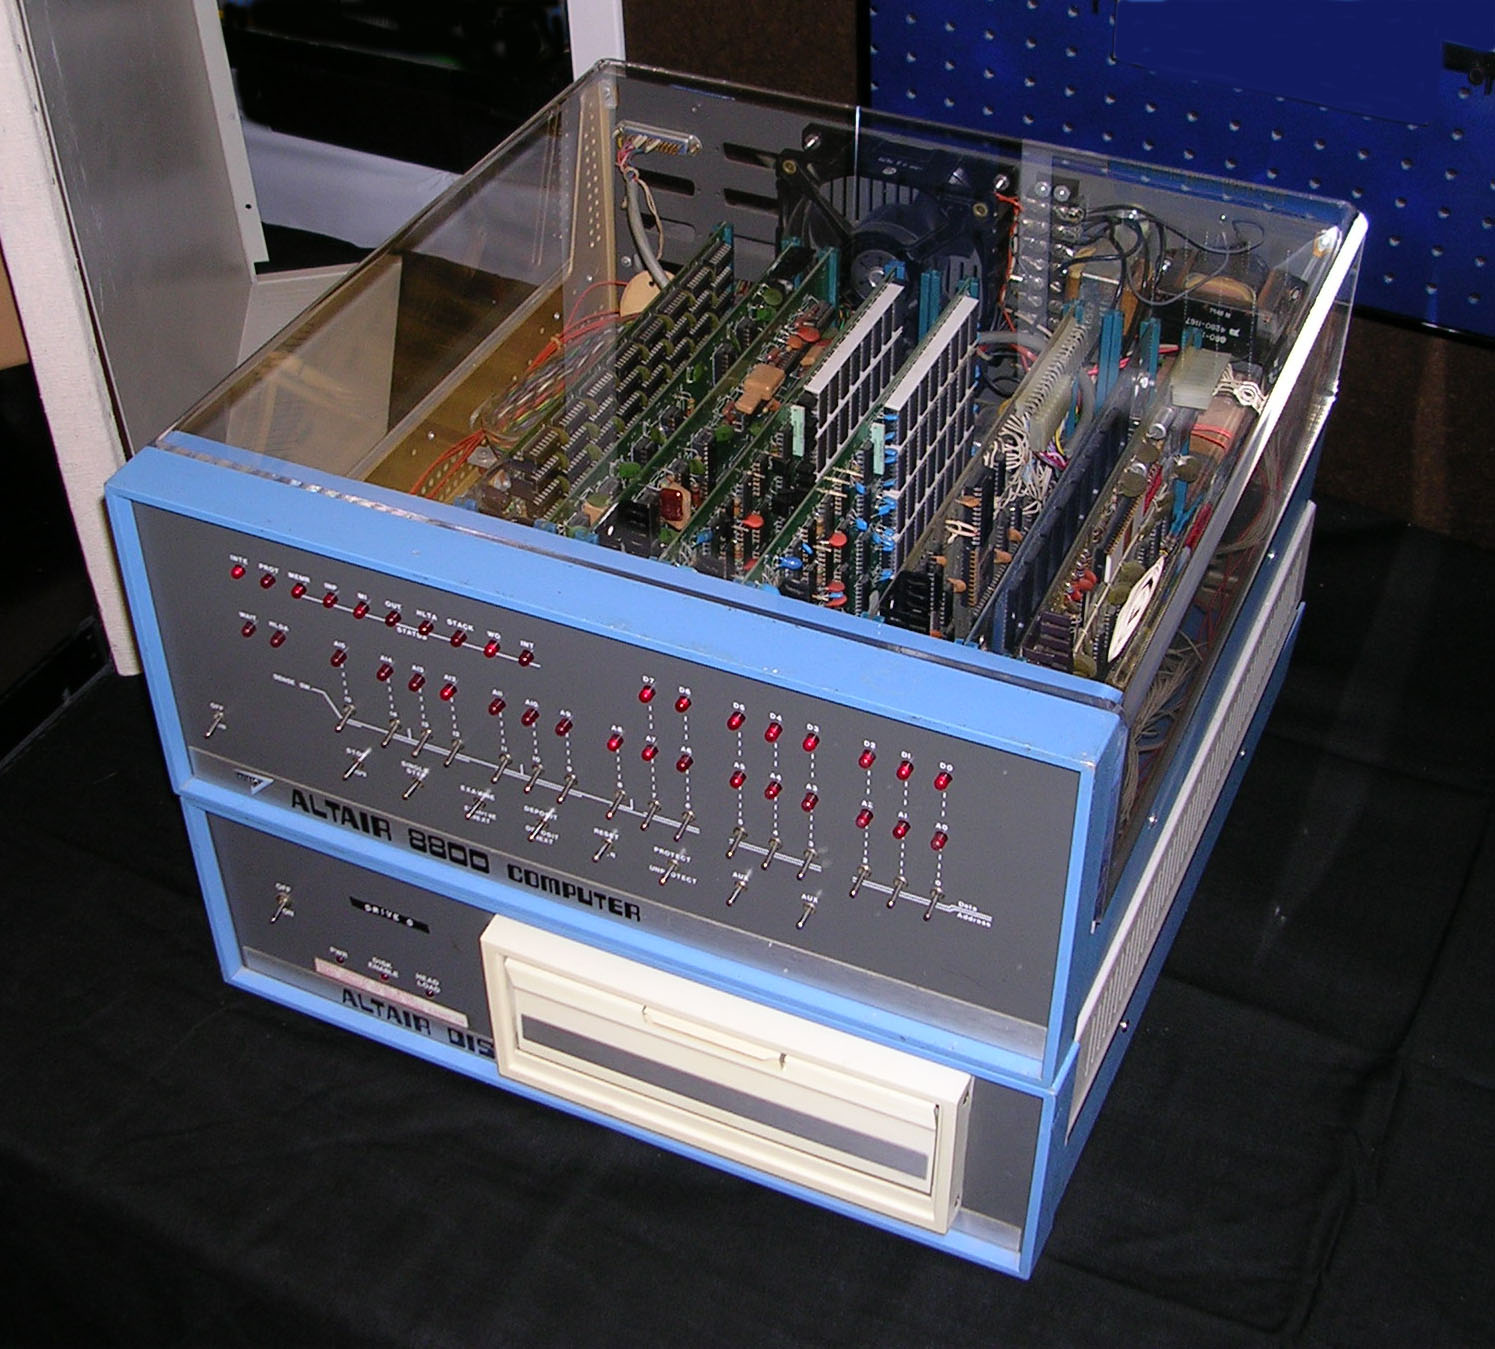
\includegraphics[width=.3\linewidth]{pics/altair_8800_computer} 
\end{center} 
\caption{MITS Altair 8800 home computer, the first market successful home computer. It used an 8-bit 8080 microprocessor and was released in 1974.\\ \textit{\small{Picture courtesy of  Michael Holley}}}
\label{Altair8800}
\end{figure}

Over the next 15 or so years, a flurry on new companies sprung up, offering a multitude of personal computers 
\cite{RN27}. New microprocessors where developed, further increasing their performance at the same time new manufacturing processes where developed that reduced their cost to manufacture. The most notably of these is the 8-bit 6502 by MOS Technology, which when released in 1975, was the least expensive microprocessor on the market by a sizeable margin 
\cite{RN40}. A sense of excitement and seemingly an expectation that computers where going to revolutionise society was abound at this time 
\cite{RN34}. Many people where having their first interactions with computers, as the home computer became more wide spread. These early home computers had a relatively simple interface, when compared to modern computers. This meant there was far less abstraction between the user and the inner workings of the computer, this may have allowed their users to more readily understand the underlying mechanisms. It also meant that users had to learn at least some rudimentary programming skills to use them. Users could get programs by typing them into their own computers out of magazines or from computer shows on TV. Most of the home computers in this period ran some form of BASIC. There where some people that questioned the usefulness of the early home computers, and with some merit, as there was a lack of software during the beginning of the era
\cite{RN23}. Others still had frankly unrealistic expectations of what computers would do for them, including doing tasks such as putting the rubbish out and babysitting. Home computers where mainly used in a four areas: business, science and engineering, education and in the home. Business, science and engineering uses included manipulating spreadsheets, word processing, basic graphics, databases and communication to connect to host computer or LANs. In the home the most widely reaching use of home computers was to play games 
\cite{RN24}. These 8-bit home computers were where many people first met and became interested in the potential of computers and computer programming and they helped kick off a revolution.


%----------------------------------------------------------------------------------------
%----------------------------------------------------------------------------------------
\section{Commodore 64, 128, 65}
\subsection{Commodore 64}
The Commodore 64 (C64) was one of the most successful home computers, selling over 17 million units according to Commodore International 
\cite{RN42}, the now defunct manufacturers of the Commodore 64. Earning it a Guinness World Record (formally Guinness Book of Records): 'Most computer sales'
\cite{RN43}.
It was first sold in January, 1982, for US\$595 at launch 
\cite{RN28}. The computational power came from a 8-bit MOS Technology 6510 microprocessor, a modified version of the 6502 mentioned in section \ref{sec: Early home computer era}. It had 64 kilobytes of RAM, which was the inspiration of its name. The Commodore 64 was a dominant market presence in its time. In a category of influential computers (home computers), the Commodore 64 may well have been the most influential of all. It ran a version of BASIC and there was a huge software library created for it during its lifetime and there's still new software being developed for the C64 to this day.
\cite{RN82}\cite{RN83}\cite{RN84}.

\subsection{Commodore 128}
The Commodore 128 (C128) was Commodore International's innovation of the very successful Commodore 64. Released in January, 1985, It was meant to build on the success of the C64 while still being near 100\% compatible with Commodore 64 software. It was powered by a more powerful 8-bit 8502 microprocessor and had 128 kilobytes of RAM. An innovation was the inclusion of a second microprocessor, an 8-bit Zilog Z80. This second CPU allowed the C128 to run CP/M (an operating system of the time) as well as the Commodore BASIC environment similar to the C64. Running CP/M allowed the C128 to access the CP/M software library, which was quite extensive, as well as the Commodore 64 software library, giving the C128 one of the broadest ranges of software compared to its competitors of the day
\cite{RN32}.

\subsection{Commodore 65}
The Commodore 65 (C65) was in development in 1990-1991, when Commodore Business Machines (subsidiary of Commodore Intentional) went bankrupt in 1994, a number of prototypes where sold on the market. It was planned to be an upgrade of the C64. \textit{Compute! Gazette} reported in an article in 1989 that the C65 had a 16-bit 65816 microprocessor; a 16-bit version of the 6502 
\cite{RN31}. Years later, when the prototypes where sold on the market by liquidators, sources report a modified 65CE02 microprocessor was used instead
\cite{RN30}
\cite{RN78}. The 65CE02 was an 8-bit CPU with a limited ability to use 16-bit instructions. It had 128 kilobytes of RAM, expandable to 1 megabyte. The C65 had a "stunning" 640x400 pixel maximum resolution 
\cite{RN31} powered by a VIC-III graphics chip. It had a C64 compatibility mode, meant to allow near 100\% compatibility with the C64 but there have been some doubts cast on this claim
\cite{RN30}. 

%----------------------------------------------------------------------------------------
%----------------------------------------------------------------------------------------
\section{History of the MEGA65 project}
Started in December 2013 by Dr. Paul Gardner-Stephen 
\cite{RN44}, the MEGA65 project is attempting to innovate the Commodore 65, with near 100\% compatibility with C64 software. Dr. Paul owned a Commodore 65 prototype between 1994-2010, he also owned a Commodore 128 through the same time and when compared, preferred the C65. Dr. Paul also loved to tinker with these computers during the 1990 and 2000s, devising ways of accelerating the C64 CPU as an example. After deciding to sell the C65 prototype to a collector for various reasons, not least of which was their ability to maintain it, Dr. Paul always had the idea of recreating the C65, and implementing some of the tricks and ideas he had worked out or heard of over the years. Then, during Dr. Paul's Ph.D studies, he learnt to program in VHDL and it seemed possible to realise this dream using the technology of FPGAs. This dream was delayed still by technological issues with the FPGA boards of the time not quite being fast enough for Dr. Paul's vision. But by 2013, a sufficient board had been released to the market. \\\\

Dr. Gardner-Stephen chose a Nexys4 development board, used by a lot of teaching institutions and designed with students in mind. This FPGA has many built in peripherals which can be used by the computer as well as its cost to performance ratio makes it ideal. The added benefit of using off-the-shelf FPGA board is that availability should be much greater compared to a PCB created just for MEGA65, which would be limited to small production runs carried out by the MEGA65 team or at their request 
\cite{RN45}.

The MEGA65 project is completely open-source with the hardware VHDL/verilog files describing the hardware and operating system software available on a public git repository 
\cite{RN17}. Dr. Gardner-Stephen's stated goals at the inception of the MEGA65 project are as follows: 
" \begin{itemize}
\item Better graphics than the Apple IIgs, Atari 800 or Plus/4: 1920x1200 @ 60Hz, 256 colour palette from 4,096 colours (later from 24-bit colour palette once I create an HDMI output) via my VIC-IV video controller.
 \item    Better sprites than the C64.  Plan is for the 8 compatibility sprites, plus perhaps 32 256-colour Enhanced Sprites with hardware scaling and practically unlimited size.  Maximum number of displayable sprites will depend on the resolution of the display and the sprites on a given raster line.
 \item    Faster CPU than the SuperCPU or any available 65C816 CPU (20MHz), and ideally with enough headroom to beat a 20MHz 65C816 running in 16-bit mode.  Currently the 65GS10 runs at 96MHz, but with an effective speed more like 48MHz until I work on some planned IPC improvements, like a 16-bit cache of zero-page to make zero-page indirect instructions take as little as 3 cycles.
 \item    More RAM than a fully expanded Apple IIgs or C65 (~8.125MB).  It will initially have 128KB of chipram like the C65, plus 16MB of slowram, plus "some" ROM.
 \item    Comparable or better sound capability than the Apple IIgs.  Multiple SIDs plus digital audio channels.  Design to be finalised.
\end{itemize} " \cite{RN45}. \\\\

After discussions to make sure their goals where aligned, In April 2015, Dr. Gardner-Stephen and MEGA.org announced a partnership to make an open-source Commodore 65-like computer 
\cite{RN47}, called the MEGA65. When asked about the motivation of the project in the press, Dr. Gardner-Stephen remarked "While It is \textit{rather} pointless, it isn't \textit{completely} pointless. It's like the difference between mostly dead and completely dead in The Princess Bride.  The MEGA65 will be fun for those for whom it is fun, which is one purpose.  Also, I intend to build and use a set of MEGA65 computers in teaching" 
\cite{RN48}.  \\\\
The core of  the MEGA65, which provides the computational power, comes from a innovation of a 4502 microprocessor design; the gs4502b (Apple released an innovation of the Apple II called the Apple IIGS, which is where the inspiration for putting GS in the name came from). In 2015 there where plans for a laptop as well as a C65-like form factor for the MEGA65, but during development the plans changed to replace the laptop with a smart phone form factor. Several other people besides Dr. Gardner-Stephen have also started working on this project; open-source community members, Flinders University students and staff. During development Dr. Gardner-Stephen also conceived of another potential use for the MEGA65, a secure device for communication and general computing, leveraging a characteristic of the MEGA65: simplicity, both in its hardware and software. This along with the open-source nature allows the MEGA65 to be completely verifiable and thus testable. Some extra features have been added and other work has been done to facilitate a secure device, which is talked about in chapter \ref{cha: Chapter 5}. The MEGA65 is currently in a prototype phase of development, most of the hardware design is complete, there are still bugs to iron out and a few feature and requirements to implement before the project moves forward.

%----------------------------------------------------------------------------------------
%----------------------------------------------------------------------------------------
\section{The progressing complexity of computer hardware and software}
The story of complexity and computers starts very much the same as the story of home computers. The technological advances led to computer hardware being smaller, faster and cheaper. At the same time, software for computers has been increasingly getting more complex. 

\subsection{History of CPU complexity}
An informed discussion on complexity in computer hardware cannot be made without mention of Moore's Law. Gordan Earle Moore, American engineer and co-founder of Intel Corporation, wrote a seminal paper in 1965 titled \textit{Cramming  More  Components  onto Integrated  Circuits} in which he observed a trend in electronics: ICs are the future of electronics and they have been getting small, faster and cheaper. He also predicted this trend would continue into 1975, and predicted the advances in ICs would power new technologies such as home computers, automatic controls for cars and 'person portable communication equipment' or mobile phones 
\cite{RN33}. In 1975, Moore wrote another paper, \textit{Progress In Digital Integrated Electronics}, revisiting his earlier prediction. In this paper he observed 'Complexity of integrated circuits has approximately doubled every year since their introduction' 
\cite{RN52}. He also predicted this would continue into the future and it largely has, as seen in figure \ref{tran_count_over_time}. 

\begin{figure} \begin{center}
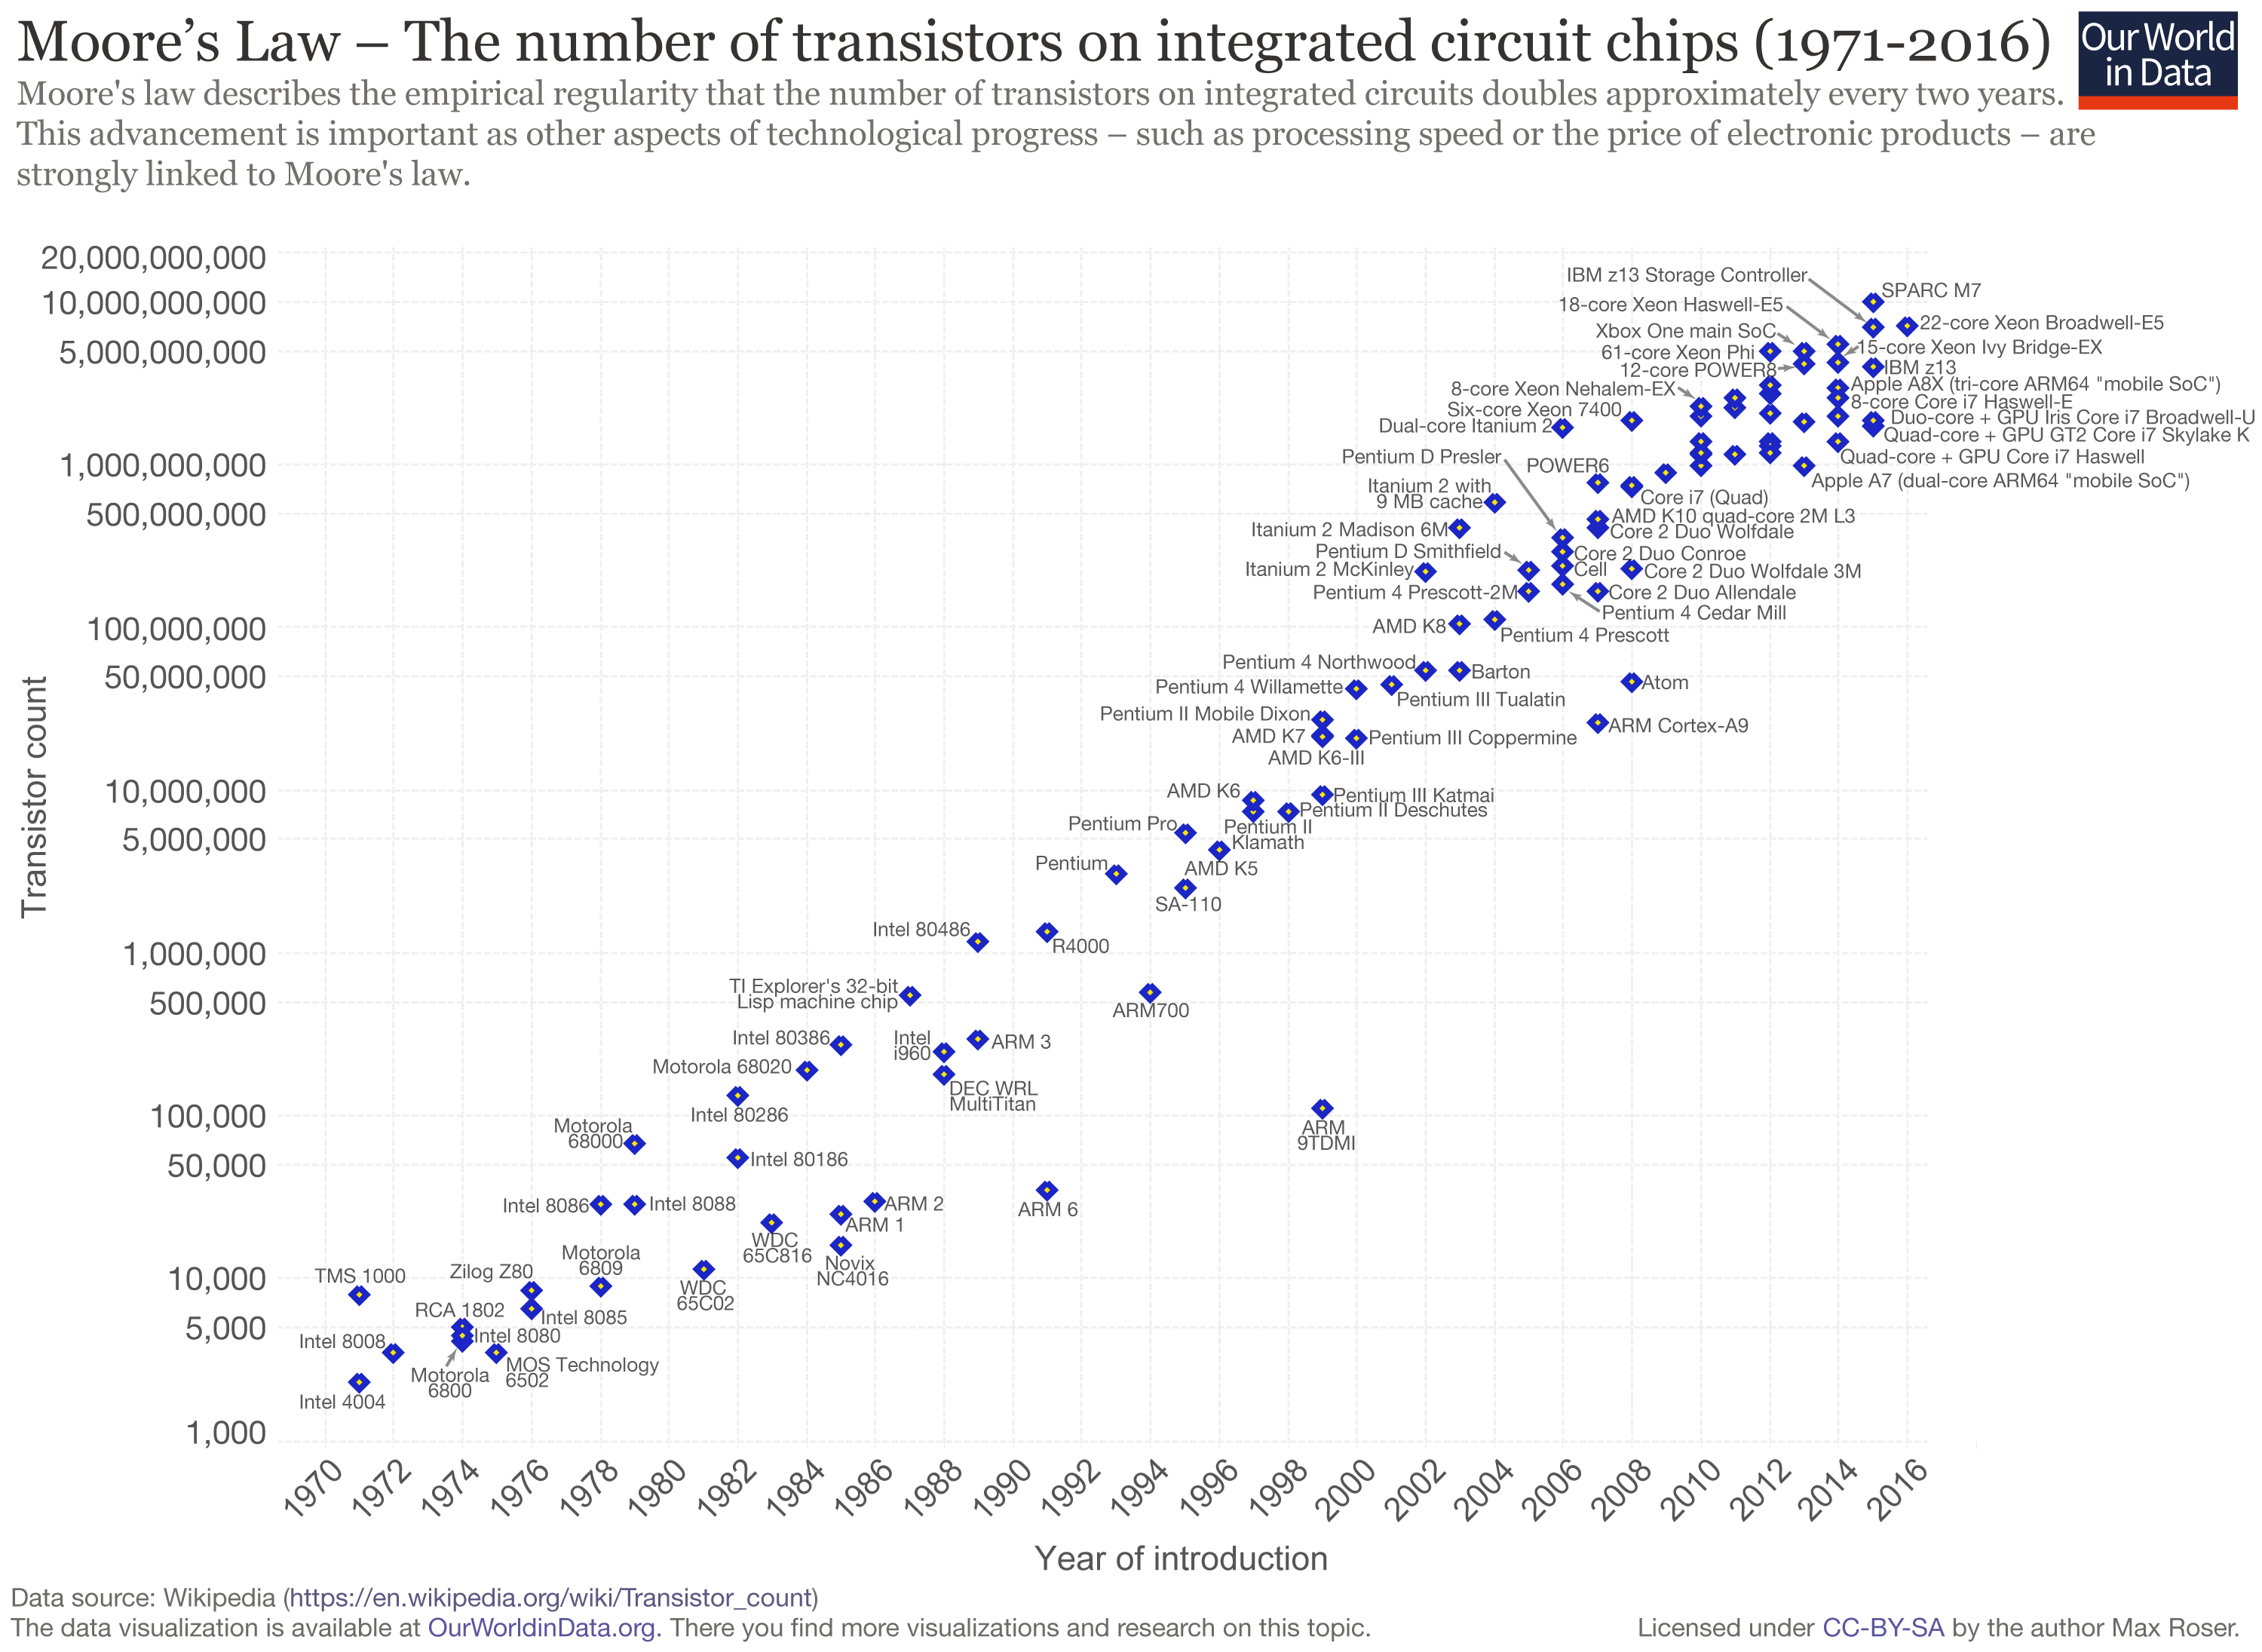
\includegraphics[width=1\linewidth]{pics/moore_law} 
\end{center} 
\caption{Plot of transistor count vs released year for microprocessors\\ \textit{\small{Picture courtesy of  Max Roser}}}
\label{tran_count_over_time}
\end{figure}

So it can been seen that transistor count has increased almost in line with Moore's prediction, with some modern CPUs having upwards of 19 billion transistors 
\cite{RN80}. But is an increase in transistor count related to an increase in complexity? Yes, they are directly proportional; by the very definition of complexity, adding more transistors to an IC would increase its complexity.

\subsection{History of operating systems complexity}

Software has also been increasing in complexity. To defend that statement a metric needs to be decided upon which can then be used to compare software from different years. Once the metric is decided, then the type of software to compare needs to be decided, as no single piece of software, to the best of the author's knowledge, has been runnable during all the years on a modern (for the relative year) CPU.

Complexity relates to how many 'things' the whole is comprised of. A piece of software is comprised of many quantifiable things: methods, lines of code etc. Which could all have justifiable reasons for being chosen. There is also several software metrics such as cyclomatic complexity that would be ideal for this task, but for reasons of practicality it was decided on using the total space in memory the software occupies when installed. This choice was made because it was the only way to get enough data to make meaningful comparisons over the span of years.

To pick what software, or class of software to compare, it was decided the comparisons should be software that is relevant to this topic, so software designed for home computers and their modern equivalents. This rules out any firmware. Various user application have been popular throughout computers history: games, word processing, spreadsheets, communication and scientific and or engineering  programs. Games, communication, science and engineering applications vary too much in their scope and function to be a reliable comparison. Word possessors and spreadsheets could be considered but again for utilitarian reasons (it was easier to find data) another form of software for home computers was used, operating systems. Even here the data is not completely reliable as it came from a wikipedia entry, an extremely well referenced wikipedia entry (191 references) but still unreliable. The disk space requirements of Windows operating systems designed for home computers (and their modern equivalents) was compared over a period of 20 years in figure \ref{win_year_size_plot}\cite{comp_win}.

\begin{figure} \begin{center}
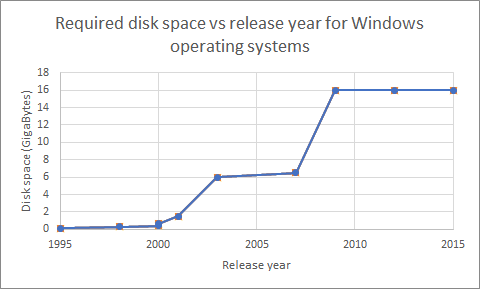
\includegraphics[width=0.8\linewidth]{pics/windows_year_size_plot} 
\end{center} 
\caption{Plot of disk space requirements to install different version of Windows operating system vs released year\\ \textit{\small{Data provided by }}}
\label{win_year_size_plot}
\end{figure}

Others have commented on this observation before. Lawson takes a broader view, talking about the complexity of computer systems as a whole and how software effects that complexity 
\cite{RN55}, as well as the rise in complexity over time. Bruce Shneider has talked about the increase in complexity and its negative effects on security. Gelsinger et al. talks about the increase in software complexity driven by the need to keep up with rapid hardware changes while designing microprocessors at Intel 
\cite{RN18}. And it would be hard to find anyone working in the industry that would disagree with the observation that software is growing increasingly complex.\\

%----------------------------------------------------------------------------------------
%----------------------------------------------------------------------------------------
\section{History of computer insecurity}
Security is described in \textit{RFC4949 Internet Security Glossary, Version 2} as a system condition where system resources are free from unauthorised access 
\cite{RN66}. In recent years computer security has been a widely discussed topic, mainly due to the damage that malicious programs, or malware, have caused. There are several Standards dealing just with this issue, which shows its importance in modern business and engineering 
\cite{RN70}\cite{RN68}\cite{RN69}. It is now common for companies to lose more from electronic theft than it is from physical theft 
\cite{RN76}. This was not always the case. It seems the inevitable fate of any new successful technology, to be manipulated by malicious actors. Computers and self-reproducing virus programs are both technologies which befell this fate, as will be discussed below.
Computer security had an interesting beginning. The terms we use today had not be ‘coined’ or where not in common usage, or even are used to mean something slightly different than they do now, such as the computer virus. So to begin, a brief discussion of the origin of some common (by today's standard) phrases. 
Bug/Debugging: In 1947 Rear Admiral Grace Murray Hopper noticed the Mark II computer she was using was outputting unexpected results and upon inspection found a moth across a relay, shorting it out \cite{RN75}. While the term bug was used in electrical engineering fields, this event is credited with popularising the terms use with computer programmers. A computer system ‘bug’ is an unexpected system behaviour. In this case the relay was shorted out, causing some unexpected behaviour. 
Virus: Fred Cohen first uses the term in his Ph.D. paper . Following on from Jon Neuman’s seminal work on self-reproducing automata, Fred wrote a seminal paper on computer viruses and coined the term ‘virus’. He gives credit to his teacher for the term.
Worm: very similar to a virus. Can run by itself where as a virus is attach to another piece of software, although this definition is also arguably incorrect as some viruses can invoke exe or fork() commands to self-reproduce. The term work is included here because it a common (if sometimes misused) term that was used to describe some of the earliest forms of self-reproducing programs.
Computer security is history is mainly a story of the development of computer viruses and their gradual adaption and then near exclusive use as malware. Following from the mathematical basis set out by Turing, Neumann begin studying his theory of automata. This theory, is generalised greatly, was a way to determine how a complex system, such as life, could come about from a reduced set of rules governing their interactions. His also considered self-reproducing automatic automata as a way to study this theory. This self-reproducing automatic automata became the starting point for Fred Cohen's seminal work on viruses Computer Viruses. Fred described viruses and how they could reproduce. He envisioned several useful way to implement them. Their way no ill intent in this work, it was not until later that other would use these ideas for nefarious uses, the computer viruses is indeed morally neutral, it is the creators which use them for good or evil. 
First worms/viruses where people trying things/ bored
US military probably was working in this field in secret. 
Things moved rapidly from here, the first publicly released viruses/worms where unleashed on the internet. It’s worth noting the this malware almost always uses some vulnerability or flaw in design of software or hardware to circumvention network security, this is a repeated aspect of these attacks and will be discussed more in the section on complexity. Things escalated quickly, viruses and computer security is huge now.
Other computer security issues and term that have been neglected so far are general related to computer viruses in at least some loose sense. Physical attack or ‘evil maid’ attacks are an where a malicious actor get physical access to a computer system. They could then potentially install some malware, virus or otherwise. Some other forms of malware so far not discussed but worth mentioning are trojan horses, named after the Greek story of Troy? These programs have two parts, a server part installed on a target computer system and a client part, used by the malicious actor to connect to the server part and then do what they want. Lure programs are programs which try to trick or deceive a user by looking like another program (Unix login lure program). Both Trojans and lures are no-self-reproducing and can form the payload of a virus. Logic bombs a programs which wait for some logic state to activate their payload, no self-reproducing and can themselves be the payload of a virus or trojan.


\subsection{Complexity as the root cause of modern malware susceptibility}
Fred Cohen talks about inability to protect against viruses in large systems.
Neumann talks about complexity, proves its an N-NP complete problem (I think it was him, have to read again).
